Solve the heat equation $u_{xx} = u_t$ on the domain $\Omega = [0, 1]$ with initial temperature distribution 
$u(x, 0) = x$, Neumann boundary condition $u_x(0, t) = 0$ at $x = 0$, and Newton's Law of Cooling 
$u_x(1, t) = -\alpha\left[ u(1, t) - T_0 \right]$ at $x = 1$.

\begin{solution}\ \\\\
    We assume the full solution $u(x, t)$ to our system is the sum of a steady state function $u_s(x)$ and a transient 
    solution $v(x, t)$. Let $L = 1$. We begin with the observation that the fact that our Neumann boundary condition 
    at $x = 0$ combined with Newton's Law of Cooling at $x = L$ imply our steady-state temperature will eventually become
    the ambient temperature $T_0$. Hence our steady-state solution is simply:

    $$
        u_s(x) = T_0
    $$

    We now solve for the transient solution $v(x, t)$.  To do so, we utilize separation 
    of variables and assume that $v(x, t)$ is the product of some function of $x$ and some function of $t$, i.e., 
    $v(x, t) = \phi(x) G(t)$. Substituting the product form of $v(x, t)$ into the heat equation yields:

    $$
        \frac{\partial^2}{\partial x^2} (\phi(x) G(t)) = \frac{\partial}{\partial t} (\phi(x) G(t))
    $$

    and hence (observing that the partial derivatives on either side reduce to standard derivatives):

    $$
        G \frac{d^2 \phi}{d x^2} = \phi \frac{d G}{d t}
    $$

    We divide both sides by $\phi G$ to find:

    $$
        \frac{1}{\phi} \frac{d^2 \phi}{d x^2} = \frac{1}{G} \frac{d G}{d t}
    $$

    Since the left-hand side depends on $x$ only and the right-hand side on $t$, the left and right sides must be equal
    to some constant, which we denote $-\lambda^2$.

    The time-dependent side therefore becomes the first-order ODE:

    $$
        \frac{d G}{d t} = -\lambda^2 G
    $$

    with solutions for any particular $\lambda$ given by:\footnote{
        We add subscripts here to $d_{\lambda}$ and $G_{\lambda}$ in order to emphasize that the exact form of the 
        function depends on the particular value which $\lambda$ takes.
    }

    $$
        G_{\lambda}(t) = d_{\lambda}e^{-\lambda^2 t}
    $$

    Similarly, the space-dependent side becomes the following second-order ODE:

    $$
        \frac{d^2 \phi}{d x^2} = -\lambda^2 \phi
    $$

    with the following general solution (where coefficient values again depend on $\lambda$):

    $$
        \phi(x) = b_{\lambda} \sin{(\lambda x)} + c_{\lambda} \cos{(\lambda x)}
    $$

    We substitute our boundary condition $0 = v_x(0, t) = \phi_x(0)$ to find:

    $$
        0 = \phi_x(0) = \lambda b_{\lambda} \cos{(0)} - \lambda c_{\lambda} \sin{(0)} = \lambda b_{\lambda}
    $$

    If we assume non-zero eigenvalues (since we recover the trivial solution otherwise), we find that $b_{\lambda} = 0$.
    At $x = L$, we substitute Newton's Law of Cooling to find:

    \begin{align*}
        u_x(L, t) &= -\alpha \left[ u(L, t) - T_0 \right] \\
        (v(L, t) + u_s(L))_x &= -\alpha \left[ v(L, t) + u_s(L) - T_0 \right] \\
        (G(t) \phi(L) + T_0)_x &= -\alpha \left[ G(t) \phi(L) + T_0 - T_0 \right] \\
        G(t) \phi_x(L) &= -\alpha G(t) \phi(L) \\
        \phi_x(L) &= -\alpha \phi(L) \\
        -\lambda c_\lambda \sin{(\lambda L)} &= -\alpha c_{\lambda} \cos{(\lambda L)} \\
        \tan{(\lambda L)} &= \frac{\alpha}{\lambda}
    \end{align*}

    Since $L = 1$, we have $\tan{(\lambda)} = \frac{\alpha}{\lambda}$ and so our transient solution is given by:

    \begin{equation}
        v(x, t) = \sum_{n=1}^{\infty}{c_n e^{-\lambda_n^2 t} \cos{(\lambda_n x)}}
    \end{equation}
    
    where $\lambda_n$ solves the transcendental equation $\tan{(\lambda_n)} = \frac{\alpha}{\lambda_n}$.

    \begin{figure}[h]
        \centering
        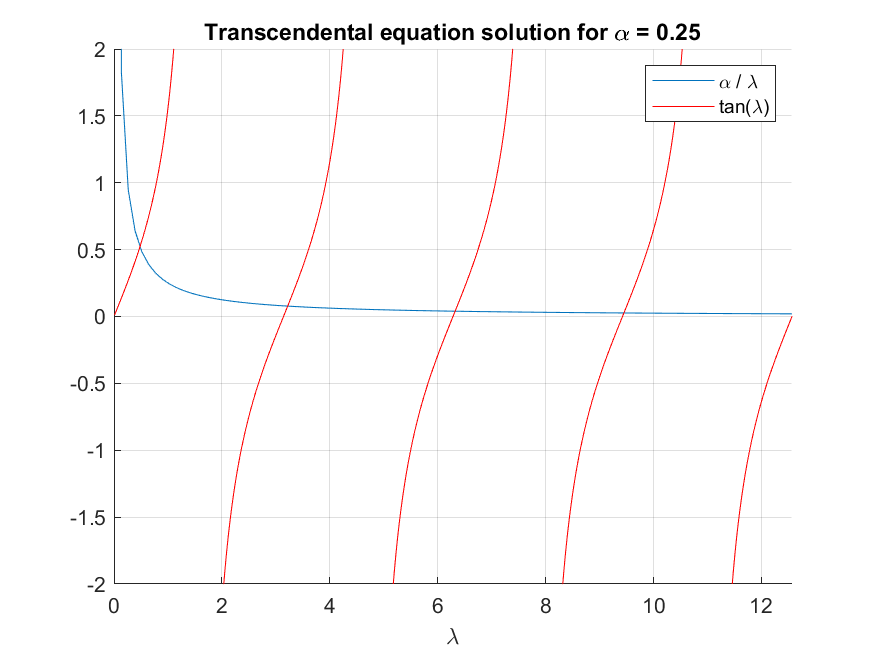
\includegraphics[width=0.7\textwidth]{problem1_transcendental_eigenvalues.png}
        \caption{$\tan(\lambda)$ and $\frac{\alpha}{\lambda}$ on $0 \le \lambda \le 4 \pi$}
    \end{figure}

    \pagebreak

    From the above plot, we see that the plots of $\tan(\lambda)$ and $\frac{\alpha}{\lambda}$ (evidently) intersect near 
    $\lambda_2 = (2 - 1)\pi$ and $\lambda_3 = (3 - 2) \pi$; in fact, as $n$ increases, we find that $\lambda_n$ gets closer
    to $(n - 1) \pi$ and so we conjecture that $\lambda_n \sim (n - 1) \pi$.

    \ \\
    To find our constants $c_n$, we first observe that our transient initial condition is given by:

    $$
        20 = u(x, 0) = u_s(x) + v(x, 0) = T_0 + v(x, 0)
    $$
    
    We solve for $v(x, 0)$ and substitute our result into (1) (letting $t = 0$) to find:

    \begin{equation}
        20 - T_0 = \sum_{n=1}^{\infty}{c_n \cos{(\lambda_n x)}}
    \end{equation}

    In order to isolate a particular $c_n$, we wish to multiply both sides by $\cos{(\lambda_m x)}$ and integrate over our domain;
    to do so, we must first show that $\cos{(\lambda_n x)}$ and $\cos{(\lambda_m x)}$ are orthogonal with respect to the integral 
    inner product, i.e., that
    \linebreak $\int_{0}^{1}{\cos{(\lambda_m x)}\cos{(\lambda_n x)}\; dx} = 0$.

    \pagebreak

    Recall first that $\cos{(\alpha) \cos{(\beta)}} = \frac{1}{2}\left( \cos(\alpha + \beta) + \cos(\alpha - \beta) \right)$
    and hence:

    \begin{align*}
        \int_{0}^{1}{\cos{(\lambda_m x)}\cos{(\lambda_n x)}\; dx} &= \frac{1}{2} \int_{0}^{1}{\cos{(\lambda_m + \lambda_n) x} + \cos{(\lambda_m - \lambda_n) x}\; dx} \\
                                                                  &= \frac{1}{2} \left[ \frac{\sin{(\lambda_m + \lambda_n)x}}{\lambda_m + \lambda_n} + \frac{\sin{(\lambda_m - \lambda_n)x}}{\lambda_m - \lambda_n} \right] \bigg\vert_{0}^{1} \\
                                                                  &= \frac{1}{2} \left[ \frac{\sin{(\lambda_m + \lambda_n)}}{\lambda_m + \lambda_n} + \frac{\sin{(\lambda_m - \lambda_n)}}{\lambda_m - \lambda_n} \right].
    \end{align*}
    To further simplify this expresion, we recall the following two sine identities:

    \begin{align*}
        \sin{(\alpha + \beta)} = \sin{(\alpha)}\cos{(\beta)} + \sin{(\beta)}\cos{(\alpha)} \\
        \sin{(\alpha - \beta)} = \sin{(\alpha)}\cos{(\beta)} - \sin{(\beta)}\cos{(\alpha)}
    \end{align*}

    Hence the left expression inside the parenthesis in the above integral evaluation becomes\footnote{
        We also substitute $\cos{(\lambda_k)} = \frac{1}{\alpha} \lambda_k \sin{(\lambda_k)}$ from our transcendental equation.
    }:

    \begin{align*}
        \frac{\sin{(\lambda_m + \lambda_n)}}{\lambda_m + \lambda_n}
        &= \frac{\sin{(\lambda_m)} \cos{(\lambda_n) + \sin{(\lambda_n)}} \cos{(\lambda_m)}}{\lambda_m + \lambda_n} \\
        &= \frac{1}{\alpha} \left[ \frac{\lambda_n \sin{(\lambda_m)} \sin{(\lambda_n) + \lambda_m} \sin{(\lambda_n)} \sin{(\lambda_m)}}{\lambda_m + \lambda_n} \right] \\
        &= \frac{\sin{(\lambda_m)} \sin{(\lambda_n)}}{\alpha} \left( \frac{\lambda_n + \lambda_m}{\lambda_m + \lambda_n} \right) \\
        &= \frac{\sin{(\lambda_m)} \sin{(\lambda_n)}}{\alpha}.
    \end{align*}
    
    We perform a similar computation on the right expression to find:

    \begin{align*}
        \frac{\sin{(\lambda_m - \lambda_n)}}{\lambda_m - \lambda_n}
        &= \frac{\sin{(\lambda_n)} \cos{(\lambda_n) - \sin{(\lambda_n)}} \cos{(\lambda_n)}}{\lambda_m - \lambda_n} \\
        &= \frac{1}{\alpha} \left[ \frac{\lambda_n \sin{(\lambda_m)} \sin{(\lambda_n) - \lambda_m} \sin{(\lambda_n)} \sin{(\lambda_m)}}{\lambda_m - \lambda_n} \right] \\
        &= \frac{\sin{(\lambda_m)} \sin{(\lambda_n)}}{\alpha} \left( \frac{\lambda_n - \lambda_m}{\lambda_m - \lambda_n} \right) \\
        &= -\frac{\sin{(\lambda_m)} \sin{(\lambda_n)}}{\alpha}.
    \end{align*}


    \pagebreak
    We substitute these results into our original integral which yields our desired result:

    \begin{align*}
        \int_{0}^{1}{\cos{(\lambda_m x)}\cos{(\lambda_n x)}\; dx} &= \frac{1}{2} \left[ \frac{\sin{(\lambda_m + \lambda_n)}}{\lambda_m + \lambda_n} + \frac{\sin{(\lambda_m - \lambda_n)}}{\lambda_m - \lambda_n} \right] \\
                                                                  &= \frac{1}{2} \left[ \frac{\sin{(\lambda_m)} \sin{(\lambda_n)}}{\alpha} - \frac{\sin{(\lambda_m)} \sin{(\lambda_n)}}{\alpha} \right] \\
                                                                  &= 0.
    \end{align*}
    
    Having shown that $\cos{\lambda_m x}$ and $\cos{\lambda_n x}$ are orthogonal when $m \neq n$, we are now ready to solve for $c_n$ in (2).
    To do so, we multiply each side by $\cos{(\lambda_m x)}$ and integrate over our domain to find:

    \begin{align*}
        \int_{0}^{1}{(20 - T_0) \cos{(\lambda_m x)}\; dx} &= \int_{0}^{1}{\sum_{n=1}^{\infty}{c_n \cos{(\lambda_n x)}} \cos{(\lambda_m x)}\; dx} \\
                                                          &= \sum_{n=1}^{\infty}{c_n  \int_{0}^{1}{\cos{(\lambda_n x)} \cos{(\lambda_m x)}\; dx} } \\
                                                          &= c_m \int_{0}^{1}{\cos^2{(\lambda_m x)}\; dx}.
    \end{align*}

    where we use the fact that $\int_{0}^{1}{\cos^2{(\lambda_m x)}\; dx} \sim \left(\frac{1}{2} + \frac{1}{2}\frac{\alpha}{(m-1)^2 \pi^2} \right)$.
    The integral on the left evaluates to:

    \begin{align*}
        \int_{0}^{1}{(20 - T_0) \cos{(\lambda_m x)}\; dx} &= \frac{(20 - T_0) \sin{(\lambda_m)}}{\lambda_m}
    \end{align*}

    and hence our Fourier coefficients $c_m$ are given by (for $m \ge 2$):

    $$
        c_m = \frac{(20 - T_0) \sin{(\lambda_m)}}{\lambda_m} \left(\int_{0}^{1}{\cos^2{(\lambda_m x)}\; dx} \right)^{-1}.
    $$

    If we let $\alpha = \frac{1}{4}$, we calculate (numerically) the following values for $\lambda_n$ and $b_n$: 

    \begin{center}
        \begin{tabular}{ ||c c c|| } 
            \hline
            $m$ & $\lambda_m$ & $c_m$                  \\ [0.5ex] 
            \hline\hline
            $1$ & 0.48        & $1.03818 (20 - T_0)$  \\ 
            \hline
            $2$ & 3.219       & $-0.04692 (20 - T_0)$ \\ 
            \hline
            $3$ & 6.323       & $0.01251 (20 - T_0)$  \\ 
            \hline
            $4$ & 9.451       & $-0.00553 (20 - T_0)$ \\ [1ex]
        \hline
        \end{tabular}
    \end{center}

    \pagebreak
    With these coefficients in hand, we plot the first four terms of the Fourier series solution for $0 \le t \le 10$
    with step size $\Delta t = 2$ and ambient temperature $T_0 = 0$:

    \begin{figure}[h]
        \centering
        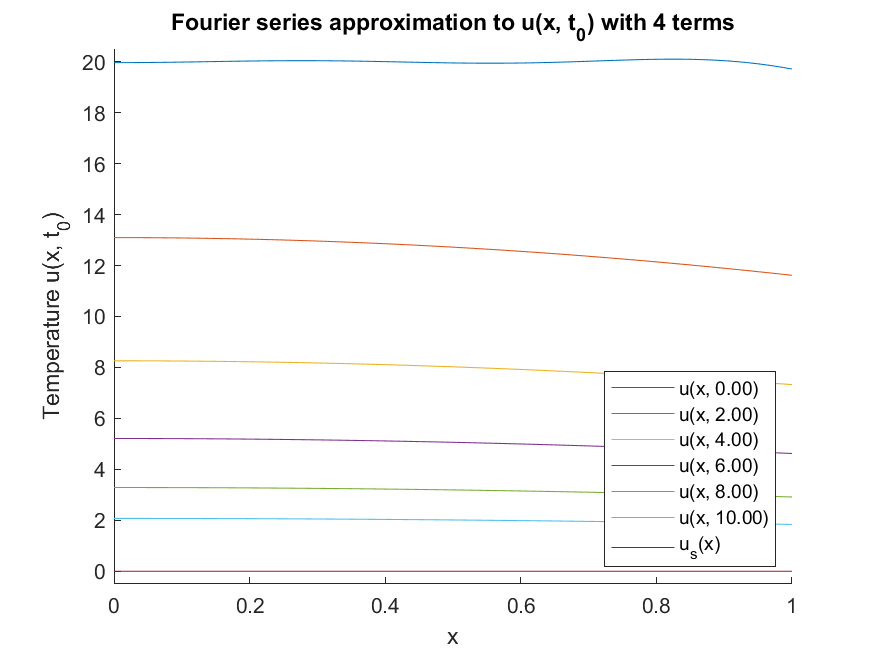
\includegraphics[width=0.7\textwidth]{problem1_fourier_series_solution_4_terms_t0_0.png}
        \caption{Fourier Series solution for $T_0 = 0^{\circ}$C}
    \end{figure}

    Observe that for small $t$, we see that the temperature is simply the Fourier series approximation to our
    initial rod temperature of $20^{\circ}$C, as expected.  In particular, we also see that the temperature 
    near $x = 1$ changes at a much higher rate than that at $x = 0$ (where it changes most slowly). This 
    observation lines up with our intuition that the temperature at a non-insulated (free) end ought to change
    rather more quickly than that at the insulated end.
    
    Furthermore, we expect the first two Fourier series terms to dominate, as we expect very little oscillatory
    behavior as the rod cools from high temperature to the low (steady state) temperature in one dimension. 
    Since the first two terms correspond to a half period greater than our right boundary at $x = 1$, these are
    the two terms which reflect a strictly cooling effect. From the table above, we see that subsequent terms 
    indeed contribute very little (and even that the effect of the second term is still relatively minor).
    
    As time progresses, we see that the intensity of the temperature decrease at $x = 1$ lessens, which we expect
    as the temperature difference term in Newton's Law of Cooling tends toward zero as the rod cools to ambient 
    temperature.

    \pagebreak
    Lastly, we note that all of the above observations hold in reverse when the ambient temperature $T_0$ is 
    greater than the initial temperature $u_0(x) = 20$ as the rod increases in temperature to $T_0$:

    \begin{figure}[h]
        \centering
        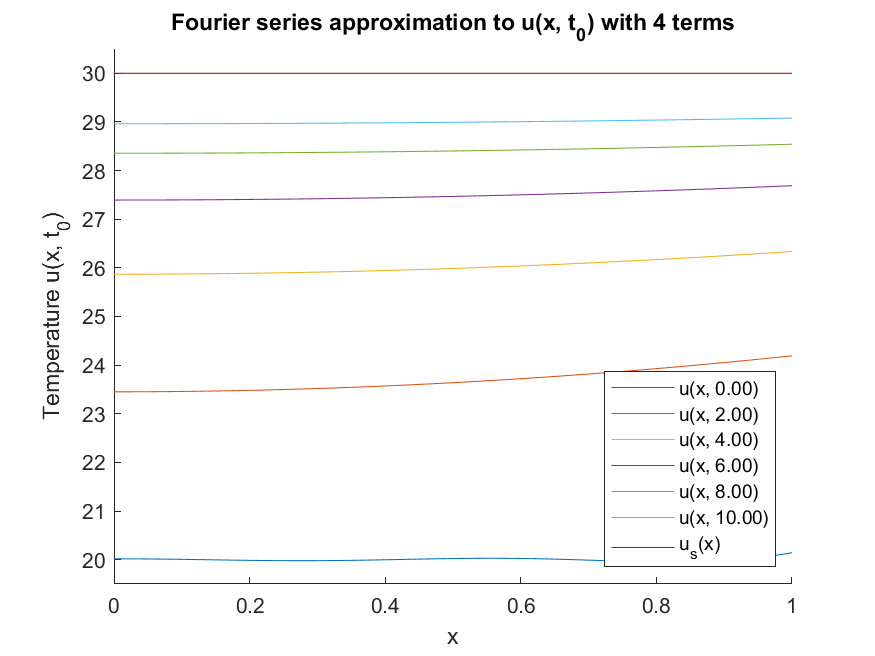
\includegraphics[width=0.7\textwidth]{problem1_fourier_series_solution_4_terms_t0_30.png}
        \caption{Fourier Series solution for $T_0 = 30^{\circ}$C}
    \end{figure}

    \pagebreak
    \textbf{Extra Credit:}\ \\

    To show that $\int_{0}^{1}{\cos{(\lambda_n x)} \cos{(\lambda_n x)}\; dx} \sim \frac{1}{2} + \frac{1}{2} \frac{\alpha}{(n - 1)^2 \pi^2}$,
    we first recall the following cosine identity:

    $$
        \cos^{2}{(\beta)} = \frac{\cos{(2 \beta)} + 1}{2}
    $$

    Our integral therefore becomes:

    \begin{align*}
        \int_{0}^{1}{\cos{(\lambda_n x)} \cos{(\lambda_n x)}} &= \int_{0}^{1}{\cos^2{(\lambda_n x)}\; dx} \\
                                                              &= \int_{0}^{1}{\frac{1}{2} + \frac{\cos{(2 \lambda_n x)}}{2}\; dx} \\
                                                              &= \left( \frac{x}{2} + \frac{\sin{(2 \lambda_n x)}}{4 \lambda_n} \right) \bigg\vert_{0}^{1} \\
                                                              &= \frac{1}{2} + \frac{\sin{(2 \lambda_n)}}{4 \lambda_n}.
    \end{align*}

    To simplify this further, we utilize the following double-angle sine identity:

    $$
        \sin{(2 \beta)} = 2 \sin{(\beta)} \cos{(\beta)}
    $$

    ...in conjunction with our transcendental equation $\sin{(\lambda_n) = \frac{\alpha \cos{(\lambda_n)}}{\lambda_n}}$ and our
    earlier conjecture that $\lambda_n \sim (n - 1) \pi$ for $n \ge 2$ to find:

    \begin{align*}
        \frac{1}{2} + \frac{\sin{(2 \lambda_n)}}{4 \lambda_n} &= \frac{1}{2} + \frac{2 \sin{(\lambda_n)} \cos{(\lambda_n)}}{4 \lambda_n} \\
                                                              &= \frac{1}{2} + \frac{2 \alpha \cos^2{(\lambda_n)}}{4 \lambda_n^2} \\
                                                              &\approx \frac{1}{2} + \frac{\alpha \cos^2{\left((n-1) \pi\right)}}{2 (n-1)^2 \pi^2} \\
                                                              &= \frac{1}{2} + \frac{1}{2} \frac{\alpha}{(n-1)^2 \pi^2}.
    \end{align*}

    Hence $\int_{0}^{1}{\cos{(\lambda_n x)} \cos{(\lambda_n x)}} \sim \frac{1}{2} + \frac{1}{2} \frac{\alpha}{(n-1)^2 \pi^2}$, as desired.\footnote{
        I did indeed like this mathematical adventure. :)
    }
\end{solution}